\documentclass[english]{article}

\usepackage{babel}
\usepackage{graphicx}
\usepackage{times}
\usepackage{pifont}
\usepackage[margin=1in]{geometry}
\usepackage{eurosym}
\usepackage{fancyhdr}
\usepackage[hidelinks]{hyperref}
\usepackage{float}
\pagestyle{fancy}
\fancyhf{}


%HEADER
%**************************************************************************************
\pagestyle{fancy}
\fancyhf{}
%**************************************************************************************
\lhead{STK600}		 	 
\rhead{Basics of Microprocessor technology} 
\lfoot{EFA12SF}
\cfoot{\thepage}
\rfoot{Nikolay Arsenov\\Alexey Tukalo}
%**************************************************************************************

\date{}
\setlength\parindent{0pt}

\begin{document}

\title{\vspace{2in}STK600\\
\small for Basics of Microprocessor technology\\
\vspace{0.5in}
\includegraphics{savonia.jpg}}

\nopagebreak
\maketitle


\vspace{3in}

\author{
\begin{flushright}
Nikolay Arsenov,Alexey Tukalo,\\
EFA12SF,\\
Information Technology,\\
Savonia University of Applied Sciences
\end{flushright}
}

\date{\today}
\thispagestyle{empty}

\newpage
\setcounter{page}{1}
\setcounter{tocdepth}{2}
\tableofcontents

\newpage

%MAIN CONTENT ******************************************************************************************************************

\section{The purpose of the STK600 card.}
The STK600 is a complete starter kit and development system for the AVR and AVR32 flash microcontrollers from ATMEL® Corporation. It is designed to give designers a quick start to develop code on the AVR. The STK600 starter kit from Atmel has a sandwich design to match a specific part package and pinout to the generic pin headers. It also features an expansion area where most part pins are available. The socket card design provides a low cost solution to support upcoming devices as the socket is the cost driving factor. 
\section{The main features}
\begin{itemize}
\item AVR Studio 4/AVR32 Studio compatible

\item USB Interface to PC for programming and control

\item Powered from USB bus or from an external 10-15V DC power supply

\item Serial In-System Programming (ISP) of AVR devices

\item JTAG programming of AVR and AVR32 devices

\item ISP and JTAG programming of AVR devices in external target systems

\item Flexible routing and socket card system for easy mounting of all supported devices

\item 8 push-buttons for general use

\item 8 LEDs for general use

\item All AVR I/O ports easily accessible through pin header connectors

\item Expansion connectors for plug-in modules and prototyping area

\item On-board 2Mbit Dataflash for non-volatile data

\item USB mini-AB (On-The-Go) connector for USB devices

\item PHY and DSUB-9 connetor for RS232 interface

\item PHY and DSUB-9 connector for CAN bus

\item PHY and header for LIN bus

\item Device board with an ATmega2560 AVR microcontroller is included. 

\end{itemize}

\section{Connecting a processor to STK600}
The box contains: 
\begin{itemize}
\item STK600 main board 
\item Cables for STK600 (two 10-wire cables for I/O ports and Parallel mode programming; one 6-wire cable for In-System Programming; four 2-wire cable for, UART and dataflash connections; USB High Speed cable; DC power cable)
\item Atmel CD-ROM with datasheets and software 
\item MCU card for ATmega2560
\item Two sets of screws and nuts, and one set of clips 
\end{itemize}
NOTE! Routing cards and socket cards for your specific device must be bought separately!!!\\\\
The system consists of a generic socket card, on which the AVR device is inserted, and a device specific signal routing card, which routes the signals from the socket pins to the different functions on the STK600 main board dependent on the device.\\\\
The STK600 starter kit is shipped with a device board with a chosen AVR microcontroller. It can be connected to the PC through the USB cable and it also can source power to the microcontroller trough that, but the power available through the USB cable is limited. If an application attaches several peripherals to the STK600, we should use an external power source connected to the DC input socket on STK600 about 9-15V DC with positive center connector.\\\\
\begin{figure}[H]
\centerline{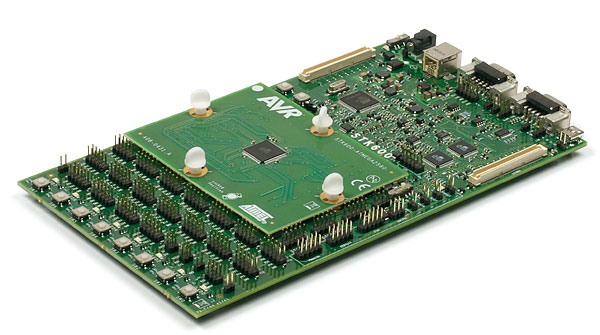
\includegraphics[scale=0.8]{MicroLab2/image001}}
\caption{STK600 board with Atmega2560 connected}
\end{figure}
The STK600 must be connected to a host PC with a USB cable and use an external power supply, for that connect the other end of the USB cable to the USB connector on STK600 sitting next to the DC jack. \\\\
The jumpers VTARGET, RESET, AREF0, AREF1 must plugged and the slider switch of the clock source must be in the position EXT.
\begin{figure}[H]
\centerline{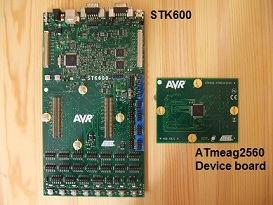
\includegraphics[scale=0.8]{MicroLab2/image002}}
\caption{STK600 and Atmega2560 separately}
\end{figure}
\subsection{PC software}
AVR Studio (Atmel Studio) has support for a range of devices in all speed grades. New AVR devices may be added in a new versions of the software. ATMEL Corporation have designed Atmel STK600 to support a variety of devices with different packages and pinouts only using in one board. There is some additional peripheral hardware included into starter kit to get started with the Atmel AVR in a starter kit package.\\\\
Atmel Studio6 is the main PC software for programming for us. It is an environment for coding with abilities to debug the programming code on a board. As we said before, STK600 supports plenty of different devices and when a user wants to start programming, there will be a dialog to create a new project, where you can choose what kind of core is correct for your future application, for example STK600 with ATmega2560 core or STK600 with ATmega128.
\begin{figure}[H]
\centerline{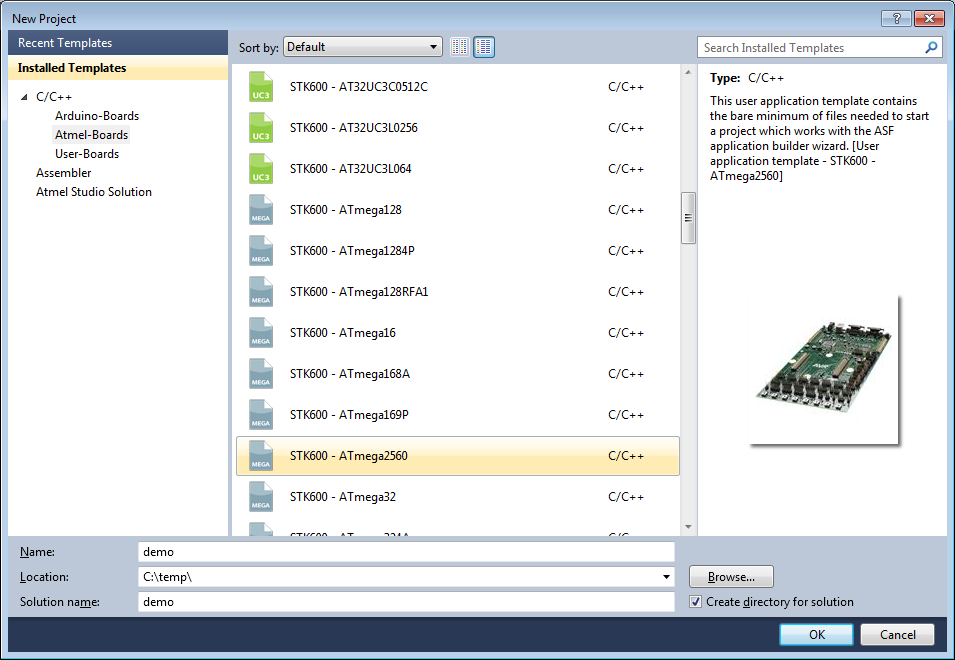
\includegraphics[scale=0.3]{MicroLab2/image021}}
\caption{Choose a correct device with necessary core}
\end{figure}
\section{The price of the development kit}
The prices are in the range form \euro 157  to \euro 227  :
\begin{itemize}
\item \href{http://store.atmel.com/PartDetail.aspx?q=p:10500155#tc:description}{store.atmel.com} - \$ 199 or \euro 157 \footnote[1]{in according with exchange rates at \today} 

\item \href{http://www.equinox-tech.com/products/details.asp?ID=1215}{equinox-tech.com} - \pounds 155 or \euro 197 

\item \href{http://www.reichelt.de/Programmer-Entwicklungstools/AVR-STK-600/3//index.html?ACTION=3&GROUPID=5514&ARTICLE=84348&SHOW=1&OFFSET=16&&SID=14UpmGeX8AAAIAAAs52Xc22cc5ced75ce22e99ee3d7b9000dabc6&LANGUAGE=EN}{reichelt.de} - \euro 227  + delivering 
\end{itemize}
We also have take in account delivering prices which are dependent form a customer's and store's locations.

\section{The parts of the card}
\begin{figure}[H]
\centerline{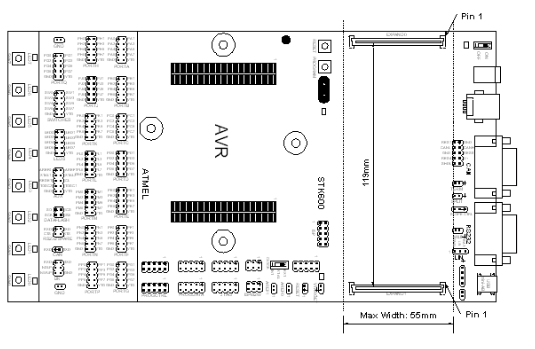
\includegraphics[scale=0.6]{MicroLab2/expansionCard}}
\caption{Expansion card slots}
\end{figure}
The expansion card (also expansion board or adapter card) is a card that is connected to the board to add functionality to the system via the expansion connectors, see Figure 4. All AVR I/O ports, programming signals and control signals are routed to the expansion connectors. The board should have a special size to be suitable. 
\begin{figure}[H]
\centerline{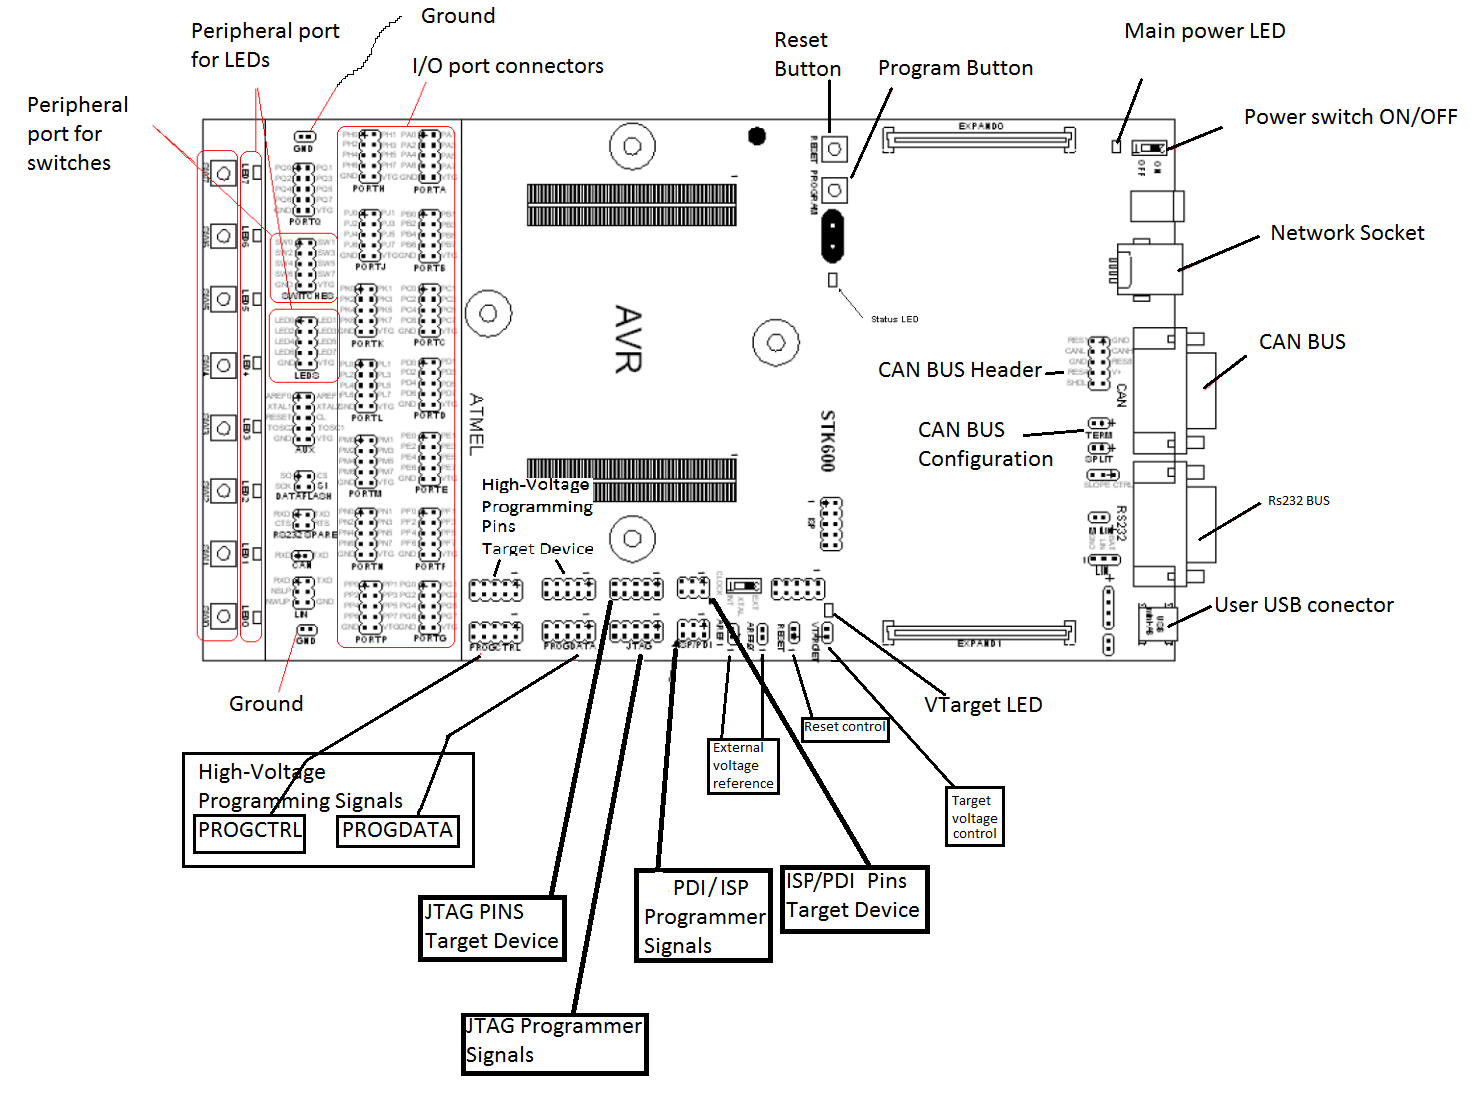
\includegraphics[scale=0.3]{MicroLab2/components}}
\caption{Components of STK600 board}
\end{figure}
Target voltage control – jumper, if removed – target voltage must be supplied from an external source. \\\\
There are three status LEDs, which shows the current state of a board, does it need to be troubleshoots or is there any errors, is there enough voltage and etc – Main Power LED (shows that board on or off depends on Power Switch ON/OFF), VTARGET LED if green – the voltage is 0.9V or higher available on the VTG, STK600 Status LED if blinking orange or slow frequency red or high frequency red – there are errors; green (READY); red (no board detected); orange (Busy programming); orange/red (upgrade mode).\\\\
Analog Reference Voltages – used by the AVR’s A/D converters to set its converting range. If the jumpers are mounted on the board, the possible analog voltage can be adjusted from the PC software in the range 0...5,5V, but not above VTARGET.\\\\
Ground – used for a supplying an external source power, else it can damage the board.\\\\
Reset jumper connects the RESET pin on the target AVR to the SRK600 and if it is mounted STK can control the RESET signal from the Reset Button, else the RESET signal is disconnected and if we will push the Reset Button – the button will not have a reset function. The RESET jumper must be always connected when user use High-Voltage programming an AVR device.\\\\
PORTA, PORTB, PORTC..etc. All of them are I/O ports pins on the target AVR used for connecting the core and peripherals on the board or external hardware. For example, a user wants to work with LEDs on a board or Switches – they are a peripherals, the user have to connect their ports to one of the PORTA/B/C or something else to have a connection between programmed processor and LEDs/Switches. Let’s connect PORTC to port LEDS and PORTB to port SWITCHES, thus while programming we can set a values to PORTC and one of the LED will blink in the output or we can use switch buttons connected to the PORTB to get how many times we pushed like the input. \\\\
CAN transceiver (Controller Area Network) is a broadcast, differentioal serial bus with high immunity to electromechanical noise.\\\\
PROGRAM Push Button – used to help AVR Studio environment to detect old software versions of STK600 and update the Flash program memory of the master MCU.\\\\
In-System Programming (ISP) uses the AVR internal Serial Peripheral Interface to download code into the flash and EEPROM memory, fuses, lockbits and signature information.\\\\
JTAG uses to debug and download the code to the board’s memory through 10-pin connector cable.\\\\
PDI programming and debugging interface is suitable for all ATxmega devices, it can download code into flash application and boot memories, EEPROM memory, fuses, lockbits and signature information. It is on the same port as ISP port.\\\\
\section{The power supply}
The USB cable can be used as source of power for STK600, but the USB cable is able to provide only limited amount of power. As result external power source is needed, if the board is extended by hardware that may need more than $300mA$. It needs $10$-$15V$ DC power supply with DC jack.\\\\
The VTG voltage is the supply voltage to the target Atmel AVR microcontroller, which is connected to the Vcc pin, it can either be generated by Atmel STK600 or supplied from an external source.\\\\
We can connect the external source to one of the VTG pins on any of the PORT headers and to the common ground (GND) when using an external VTG voltage. If we use VTG voltage, it have to be larger than any of the AREF (reference voltages) and the STK600 must always be powered on, else the kit may become damaged.  
\begin{figure}[H]
\centerline{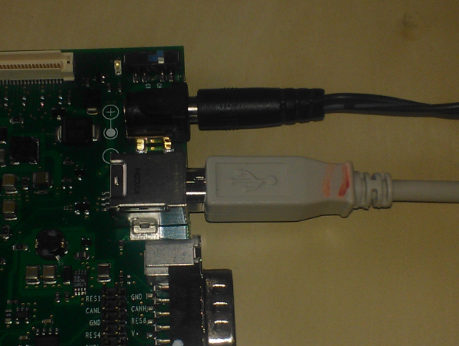
\includegraphics[scale=0.8]{MicroLab2/image011}}
\caption{Powering STK600}
\end{figure}
\section{Cenecting IO devices}
 \begin{figure}[H]
\centerline{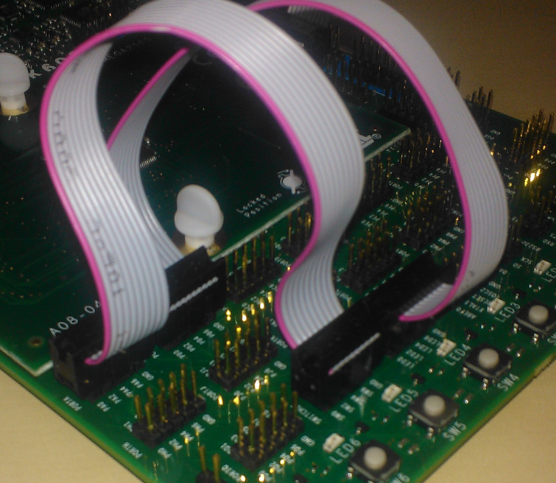
\includegraphics[scale=0.8]{MicroLab2/image009}}
\caption{I/0 switches and leds connection}
\end{figure}
In the STK600 board there are I/O ports like PORTA, PORTB and etc, which are connected to the processor and used for programming signals in a code, these kind of ports can be connected with peripheral devices, such as LEDs or Switches. LEDs peripheral has its own separate port named LEDS and peripheral for Switches also has its own port named SWITCHES. These peripheral ports have a special functionality to get the signals from the processor through I/O ports and send it to the LEDs or for example get a signal from Switches like an input and send the signal to the processor through the I/O ports. In the Figure 7 we can see the connection of PORTA with LEDs port and PORTB connected with SWITCHES port through 10-pins wire. In our application code a programmer has to program PORTA as the output and PORTB as the input; send signal through PORTA and get through PORTB.  
\section{The clock setting of the processor}
There are several clock options in STK600 configuration. A switch on the board controls the following three options:
\begin{itemize}
\item Programmable clock generator
\item Crystal oscillator
\item XTAL1 Pin tri-stated
\end{itemize}
\subsection{Programmable clock generator}
PC software is able to set programmable clock generator with frequency in the range from $1kHz$ to $32MHz$ with 0.5\% accuracy.
\subsection{Crystal Oscillator}
XTAL position of the CLOCK switch sets a crystal oscillator as a clock source. The on-board crystal produces frequency form $4MHz$ to $24MHz$. The crystal should be placed in the socket.
\subsection{XTAL1 Pin Tri-stated}
AVR can also run on the internal oscillator, and in this case the XTAL1 connection  pin from the clock source on STK600 is not compulsory. The CLOCK switch should be set to the INT position.
\subsection{Real Time Clock} 
The STK600 also has 32768 Hz oscillator, the feature can be used to make real time clock. A pin on the AUX header contains the $32KHz$ output from the oscillator. Jumper between the 32KHz and TOSC1 pin on the AUX header is able to rout the clock to the TOSC1 pin.

\section{Programming the card}
Atmel Studio6 is a software for programming AVR devices, if click on the device programming icon we can select an interface used for the programming. 
 \begin{figure}[H]
\centerline{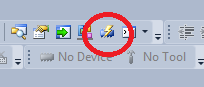
\includegraphics[scale=0.8]{MicroLab2/image014}}
\caption{programming icon}
\end{figure}
As it was said previously about different programming interfaces, we can use plenty of them for debugging or uploading a code directly to the memory. If we would like to debug the code step by step, it is better to use JTAG as the interface.
 \begin{figure}[H]
\centerline{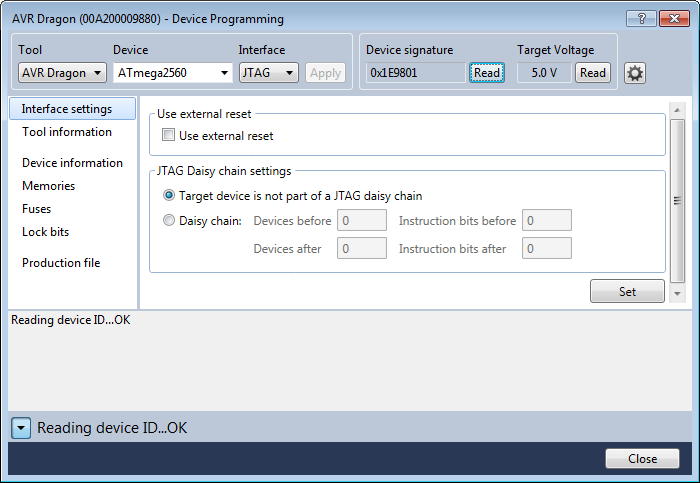
\includegraphics[scale=0.5]{MicroLab2/image015}}
\caption{Select AVR Dragon as the programmer and JTAG as the interface, then click on Apply. AVR Dragon Used for debugging the program.}
\end{figure}
On the other hand, we can use ISP - the AVR internal Serial Peripheral Interface to download code into the flash and EEPROM memory, fuses, lockbits and signature information. For that we have to click on the same button – connect device, then select Memories and Program. And the code will be uploaded to the device and ready to use, but we cannot use debugging in this way.\\\\
One more way is using PDI programming and debugging interface is suitable for all ATxmega devices, it can download code into flash application and boot memories, EEPROM memory, fuses, lockbits and signature information. It is on the same port as ISP port.

\section{ISP - programming}
ISP (Serial Peripheral Interface)  is able to program as flash as EEPROM memory of an AVR it also can change settings of fuses, lockbits and calibration bytes. ISP connection contains only three pins:
\begin{itemize}
\item VCC
\item GND
\item RESET
\end{itemize}

The ISP frequency (SCK) can be set on the AVR Studio and must be less then 25\% of the target clock.

\section{Default settings}
As it was said before, some jumpers used to add some functionality to the buttons or to work as transistors – to save the card from the damage. \\\\
In the beginning of work with STK600, there must be plugged some jumpers. For example, Reset jumper connects the RESET pin on the target AVR to the SRK600 and if it is mounted STK can control the RESET signal from the Reset Button, else the RESET signal is disconnected and if we will push the Reset Button – the button will not have a reset function. The RESET jumper must be always connected when user use High-Voltage programming an AVR device.\\\\
Or there is another jumper is the VTARGET jumper, which answer for external power source to STK600. If the VTARGET jumper is removed, VTG must be supplied from an external source. If we use VTG voltage, it have to be larger than any of the AREF (reference voltages) and the STK600 must always be powered on, else the kit may become damaged.\\\\
The jumpers AREF0, AREF1 must plugged to set the reference voltage to the card, used for ADC conversions, and the slider switch of the clock source also must be in the position EXT.
 \begin{figure}[H]
\centerline{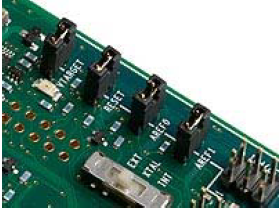
\includegraphics[scale=0.8]{MicroLab2/image010}}
\caption{Default jumpers}
\end{figure}
\end{document}
